\chapter{Návrh vzorovej sady grafických komponentov}

V programe Inkscape som vytvorila nasledujúcu sadu grafických komponentov. Vzorová sada grafických komponentov SCADA systémov obsahuje:
\begin{itemize}
	\item Prečerpávacia stanica - obrázok \ref{fig:pump} umožňuje meniť indikátor prítoku na červenú alebo zelenú. Je možné spustiť alebo zastaviť rotáciu motora a animovať stúpanie a klesanie hladiny v nádrži. 
	\item Prepravný pás - obrázok \ref{fig:belt} znázorňuje pohyb elementu po páse, pričom sa dá meniť pozícia elementu od 0 po 100 udaná v percentách. 
	\item Trojcestný ventil - obrázok \ref{fig:trippleValve} znázorňuje dva motory, ktoré sa dajú spustiť a zastaviť, čo je znázornené rotáciou vrtuliek. Ak je ventil zelený, je otvorený a ak je červený, tak je zatvorený a nepriepustný.   
	\item Mapa Slovenska - obrázok \ref{fig:map} umožňuje zmenu farby jednotlivých krajov, pridanie a zmeny farby textu, umožňuje pridať element na predefinovanú cestu a animovať pohyb medzi jednotlivými bodmi. 
	\item Thermometer - obrázok \ref{fig:thermometer} animuje pohyb stúpania alebo klesania teploty na určitú hodnotu. Hodnota sa zadáva v percentách. 
\end{itemize}

Vytvorila som interface metód, ktoré majú obsahovať jednotlivé grafické komponenty. Sú zobrazené v diagrame tried, ktoré sú na obrázku \ref{fig:classD}


\begin{figure}[hp]
	\centering
	\includegraphics[width=0.9\linewidth]{uml/classDiagramTried.png}
	\caption{Diagram tried vzorovej sady grafických komponentov}
	\label{fig:classD}
\end{figure}


\begin{figure}[H]
	\centering
	\includegraphics[width=0.7\linewidth]{obrazky/pump}
	\caption{Prečerpávacia stanica}
	\label{fig:pump}
\end{figure}
%%%%%%%%%%%%%%%%%%%%%%%%%%%%%%%%%%%
\begin{figure}[H]
	\centering
	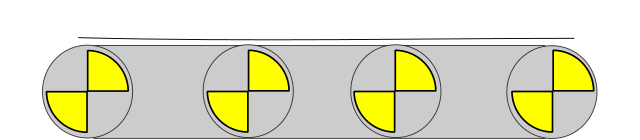
\includegraphics[width=0.7\linewidth]{obrazky/belt}
	\caption{Prepravný pás}
	\label{fig:belt}
\end{figure}
%%%%%%%%%%%%%%%%%%%%%%%%%%%%%%%%%
\begin{figure}[H]
	\centering
	\includegraphics[width=0.7\linewidth]{obrazky/trippleValve}
	\caption{Trojcestný ventil}
	\label{fig:trippleValve}
\end{figure}
%%%%%%%%%%%%%%%%%%%%%%%%%%%%%%%%%%%%%%%%%
\begin{figure}[H]
	\centering
	\includegraphics[width=0.7\linewidth]{obrazky/map}
	\caption{Mapa Slovenska}
	\label{fig:map}
\end{figure}
%%%%%%%%%%%%%%%%%%%%%%%%%%%%%%%%%%%%%%%%%
\begin{figure}[H]
	\centering
	
\includegraphics[width=0.2\linewidth]{obrazky/thermometer}
	\caption{Termometer}
	\label{fig:thermometer}
\end{figure}